\subsection{Abbildungen}

\subsubsection{Definition}
Seien A und B zwei Mengen.
Dann ist eine \emph{Abbildung} ein eindeutige Vorschrift, die jedem Element aus A genau ein Element aus B zuordnet.
Ein andere Bezeichnung für Abbildung ist \emph{Funktion}.
\subsubsection{Beispiel}
Sei $f:{A}\longrightarrow{B}$ eine Abbildungsvorschrift.
Dann ist:
\begin{align*}
   ker(f) := \{(a,c) \in A \times A\ | f(a)=f(c)\}
\end{align*}
eine Menge, der sogenannte Kern von f.

D.h. die Abbildung erzeugt sämtliche Paare von Elementen aus A, die den selben
Funktionswert besitzen. \footnote{Ich hoffe das stimmt auch, korrigiert mich hier bitte wenn
  ich das falsch verstanden habe!}
\newpage
\subsubsection{Typen von Abbildungen}
Seinen A und B zwei Mengen und $f:{A}\longrightarrow{B}$ eine Abbildungsvorschrift.
Dann gibt es 3 besondere Typen von Abbildungen:

\begin{description}
\item[surjektive Abbildung] \emph{alle} Elemente von B mindestens einmal erfassen
\item[injektive Abbildungen] alle Elemente von A erhalten \emph{unterschiedliche} Elemente aus B
\item[bijektive Abbildungen] \emph{surjektiv und injektiv} zu gleich: alle A erhalten genau ein B und alle B werden getroffen.
Dies impliziert die Umkehrbarkeit der Funktion. Eine Sonderform der bijektiven
Abbildung ist die \emph{Identität}. Dabei wird jedes Element sich selbst zugeordnet.
\end{description}

\begin{figure}
\subfigure[surjektive
Abbildung]{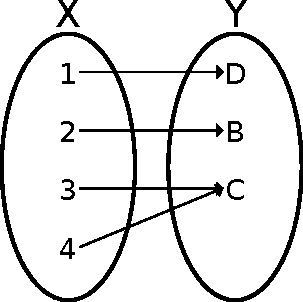
\includegraphics[width=3cm]{../bilder/Surjection.pdf}}\hfill
\subfigure[injektive
Abbildung]{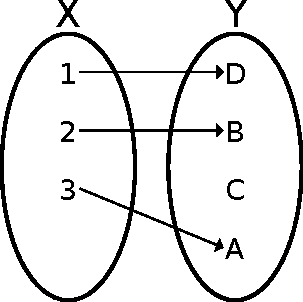
\includegraphics[width=3cm]{../bilder/Injection.pdf}}\hfill
\subfigure[bijektive
Abbildungen]{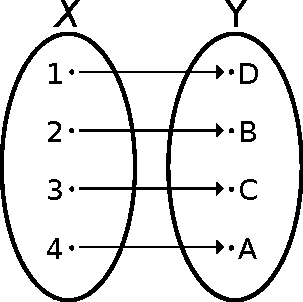
\includegraphics[width=3cm]{../bilder/Bijection.pdf}}\hfill
\subfigure[identische
Abbildungen]{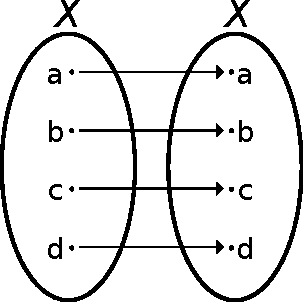
\includegraphics[width=3cm]{../bilder/Identitaet.pdf}}
\end{figure}

\subsubsection{Mächtigkeit einer Abbildung}
Seien A und B Mengen.
Dann bezeichnet $B^A$ oder $Map(A,B)$ die Menge aller Abbildungen von A nach B.
\subparagraph*{Satz:}
Für A, B endliche Mengen gilt:
$$ |B^A| = {|B|}^{|A|} $$